\section{Dynamics of Stars near the Galactic Centre}
\begin{quotation}
	\raggedleft \it The computer can't tell you the emotional story. \\ It can give you the exact mathematical design, \\
	but what's missing are the eyebrows. \\ -- Frank Zappa
\end{quotation}
The best way to probe a distribution of mass when it does not emit very strongly, is to observe the orbits of objects moving
through that distribution. Luckily the orbits of stars near the centre of the galaxy have been spatially resolved
\cite{ref_ghezorbits, ref_eckartorbits} and we may therefore use this data to compare with motion predictions from computer
simulations using the fermion ball mass distribution. But as there are a lot of stars neighbouring the central object, we must
first decide which to concentrate our efforts upon. Throughout the calculations, we assume that the central object is incident
with the radio source Sgr A*, and use 16keV, $g_\nu=2$ fermions.

\subsection{Closed and Precessing Orbits}
By nature, a point source object will produce a closed orbit, whereas a mass distribution will in general produce a precessing open orbit.
This precession is clearly a definite way to tell (over time) if the stars near Sgr A* are orbiting around a central black hole or within a mass
distribution. In order for this method of discernment to be valid, the stars must move within the fermion ball. In addition,
the stars must not possess velocities greater than the escape velocity of the black hole.
For clarity, black hole solutions are often abbreviated to BH and those of the fermion ball to FB. The escape velocity
(escape to infinity) is given by
\begin{equation}
	v_{esc}=\sqrt{2 \Phi }
	\label{eqn_escapevelocity}
\end{equation}
while the circular velocity is
\begin{equation}
	v_{cir}=\sqrt{\frac{G M(r)}{r}}
	\label{eqn_circularvelocity}
\end{equation}
Using data from \cite{ref_ghezmotion} made in 1996.58, Figure \ref{fig_escapevelocities} shows the observed velocities from
proper motion analysis alongside the calculated escape and circular velocities for the black hole and fermion ball scenarios.

There are two schools of thought on the naming conventions of the stars near Sgr A* \cite{ref_ghezorbits, ref_eckartorbits}, and the
numbers often contradict (e.g. S0-4 is also S8). We shall use the 2-digit notation where the first number
suggests the distance band which the star falls within, e.g. S0-1, S0-2... are all within $1"$ of Sgr A*, and S1-1, S1-2... within
the $1"$ to $2"$ range, and so on.
\begin{figure}[!tb]
	\begin{center}
	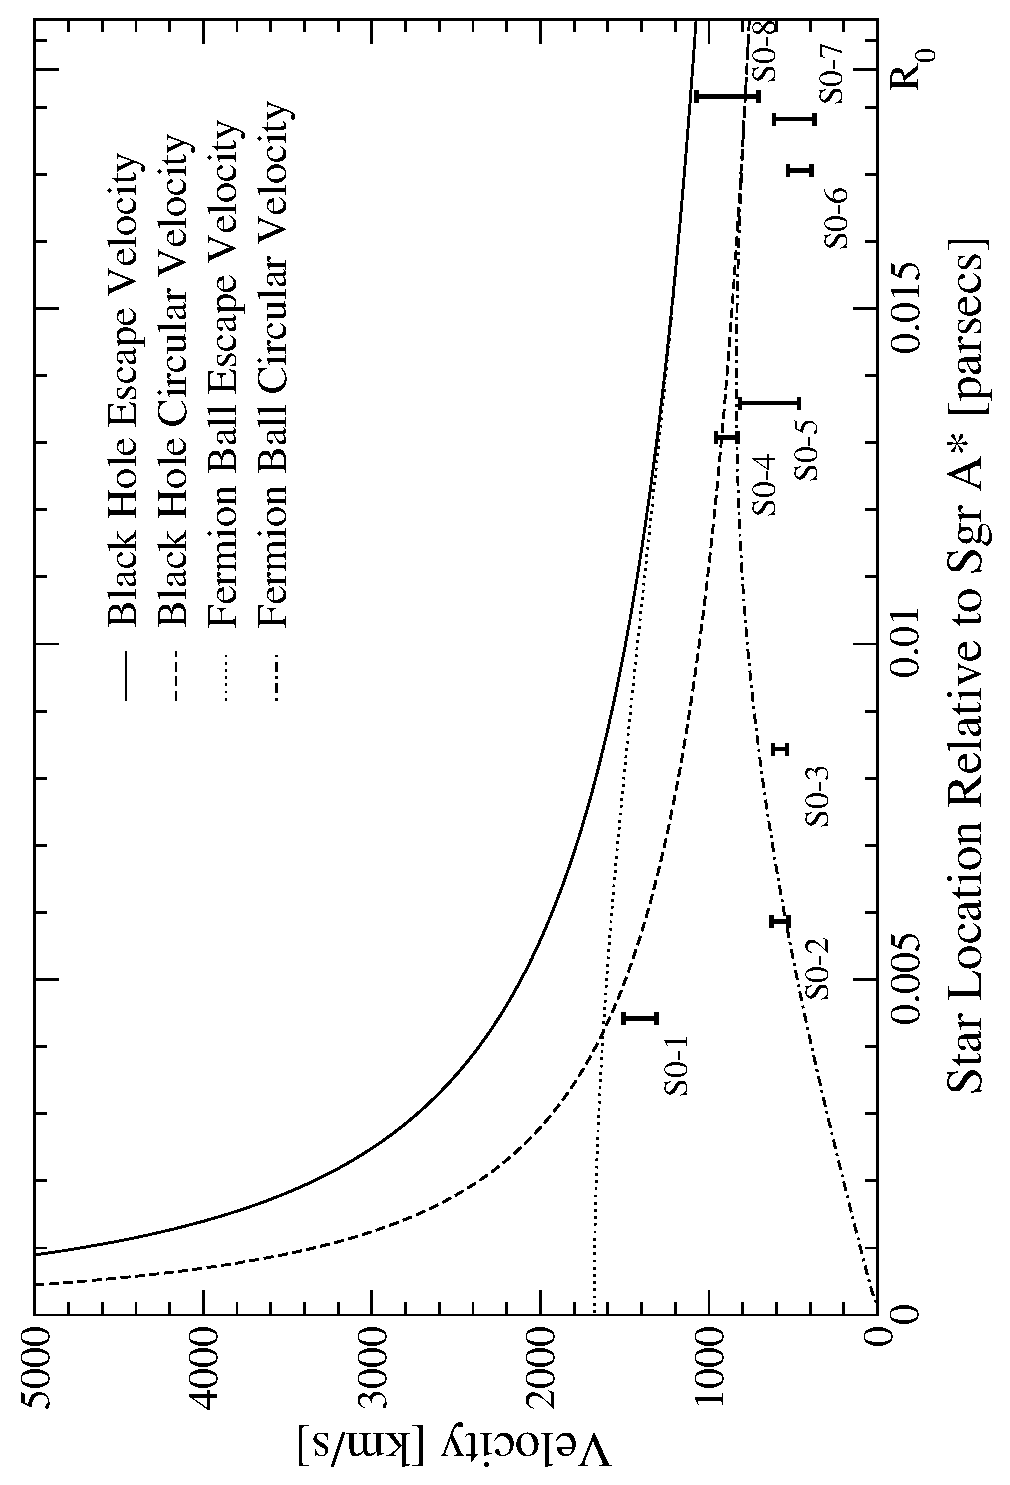
\includegraphics[angle=-90,width=0.9\textwidth]{eps/escapevelocitieswithdata.eps}
	\caption{Velocities from proper motion analysis \cite{ref_ghezmotion} alongside the calculated escape and circular
	velocities for the black hole and fermion ball scenarios. Fermion ball radius noted as ${\rm R_0}$.
	This plot is made using the position and velocity vectors as calculated from the right ascension and declination data. There
	is no data available in our line of sight, thus all points are minimal values. Epoch 1996.58.}
	\label{fig_escapevelocities}
	\end{center}
\end{figure}

S0-3 is suspected to have a very large position component in our line of sight (due to it's near `straight line' trajectory)
and is therefore ruled out as an object of interest.
However, from Figure \ref{fig_escapevelocities} it is clear that the stars S0-1 through S0-5 may be within the projected radius
of the fermion ball. However, of those stars, only S0-1, S0-2 and S0-4 have been identified as being on accelerating orbits.
We will therefore use these 3 stars to draw comparisons with models of motion.

\subsection{Newtonian Motion}
We calculate the trajectories of the stars by solving Newton's equations of motion in 3-dimensions
\begin{eqnarray}
	\frac{d^2x}{dt^2} = - \frac{G M(r)}{\left(x^2 + y^2 + z^2\right)^{\frac{3}{2}}}x \nonumber \\
	\frac{d^2y}{dt^2} = - \frac{G M(r)}{\left(x^2 + y^2 + z^2\right)^{\frac{3}{2}}}y
	\label{eqn_newtonmotion} \\
	\frac{d^2z}{dt^2} = - \frac{G M(r)}{\left(x^2 + y^2 + z^2\right)^{\frac{3}{2}}}z \nonumber
\end{eqnarray}
where $x$, $y$, $z$ are the distances from the origin in a Euclidean coordinate system centred on Sgr A*,
taking $x$ to be opposite the observed right ascension, $y$ as the observed declination, and $z$ to be the line of sight in the
direction of the sun.
The solution of the coupled differential equations (\ref{eqn_newtonmotion}) depends upon 7 initial conditions, which are the $x$, $y$, $z$
position and velocity components with the mass of the central object as the final parameter. We first minimise the fit to initial $x$, $y$
position and $v_x$, $v_y$ velocity parameters, then run a $\chi^2$ phase space analysis on the $z$ position and velocity parameters.
The effect of varying the central mass is briefly discussed afterwards using limits imposed by \cite{ref_ghezmotion}.

The data we choose to use consists of a combination of spatial analysis from 2 independent sources \cite{ref_ghezorbits, ref_eckartorbits}
on the 3 stars S0-1, S0-2 and S0-4 over the observing period 1992.7 to 2000.5. The location of Sgr A* moves over time (against the background),
fortunately the data has already considered this and all positions are relative to the location of Sgr A*. There are 36
data points for each star from 18 separate observations, which must be fitted. It is important to stress that the parameters already
mentioned as initial conditions are for the 1992.7 epoch, and cannot be directly compared, to say, the data in Figure
\ref{fig_escapevelocities}, which is the epoch 1996.58.

\subsection{$\chi^2$ Reduction of $z$ and $v_z$}

\subsubsection{Notes on $\chi^2$}
A $\chi^2$ analysis is the most commonly accepted method for comparing experimental data to a theoretical model, a smaller value
signals a better fit to the experiment. A $\chi^2_{ndf}$ ($\chi^2$ per number of degrees of freedom) is a more rigorous way to examine the fit
as it will also consider the number of data points used and the number of free variables in the theory. The form of the data in this
case is such that we must perform a separate $\chi^2$ fit for both the $x$ and $y$ observed data, each given by
\begin{eqnarray}
	\chi^2_x &=& \sum_{i=1}^{N} \frac{\left(x_i-\overline{x}(x,v_x,y,v_y,z,v_z,M)\right)^2}{\sigma^2_{x_{err}}}
	\label{eqn_chisquarex} \\
	\chi^2_y &=& \sum_{i=1}^{N} \frac{\left(y_i-\overline{y}(x,v_x,y,v_y,z,v_z,M)\right)^2}{\sigma^2_{y_{err}}}
	\label{eqn_chisquarey}
\end{eqnarray}
These $\chi^2$ values can safely be added linearly as the nature of $\chi^2$ is such that it need not be added in quadrature (as the
$\chi$ itself will already be added in quadrature). The total $\chi^2$, which is the quantity of interest can then be written as
\begin{equation}
	\chi^2 = \chi^2_x + \chi^2_y
	\label{chisquare}
\end{equation}
and the $\chi^2$ per number of degrees of freedom is
\begin{equation}
	\chi^2_{ndf} = \frac{\chi^2}{N-N_p}
	\label{chisquarendf}
\end{equation}
where $N=36$ and $N_p=7$.

Simulations of star dynamics were performed several times in order to minimise the $\chi^2$ for initial parameters $x$, $v_x$, $y$
and $v_y$, but by no means have the $\chi^2$ been fully reduced. Computing time restricted the iterations of the simulations to 4
passes, and further iterations would most certainly produce slightly smaller $\chi^2$.

The astronomical unit of arcsec has been preferred in the presentation of the results as this is the unit used during observations.
This unit system may appear unusual when referring to the $z$ axis which is in the observer's line of sight, but it can be thought
of as being equivalent to the distance projected at a fixed distance of 8kpc, as can the $x$ and $y$ axis.

\subsubsection{Best Fits}
\label{bestfits}
By first minimising the initial $x$ and $y$ position and velocity parameters, this allows for a $\chi^2_{ndf}$ phase space plot of the
unknown $z$ position and velocity parameters. Table \ref{tab_minimalzvzchisquare} lists the minimal $\chi^2_{ndf}$ for each
of the 3 stars in each scenario. Figures \ref{fig_so1BHphasespace} through \ref{fig_so4FBphasespace} are the phase space plots, using
colour as the 3rd dimension. In order to ensure a high resolution in the data representation, each plot is a result of 22,000 runs of
the simulation. There has been no interpolation performed on the images.

Table \ref{tab_minimalzvzchisquare} reveals that the fits for S0-1 have a much higher $\chi^2_{ndf}$ compared with S0-2 and S0-4.
This is due to inconsistencies within the experimental data. Figures \ref{fig_so1bestfits} through \ref{fig_so4bestfits} show the
$x$ and $y$ paths of the stars for each of the reduced $\chi^2_{ndf}$ scenarios. Extra paths are also shown for bound orbits,
where the minimum fit $\chi^2_{ndf}$ is an unbound orbit. These tables highlight the numerically minimal $\chi^2$ values for each plot,
but as can be seen clearly from figures \ref{fig_so1BHphasespace} through \ref{fig_so4FBphasespace}, the minimal $\chi^2$ is not always
well defined and the $z$, $v_z$ values may take on a much larger range only expressible in the plots.

The inconsistencies within the S0-1 data can be clearly seen in Figure
\ref{fig_so1bestfits}, possibly due to the discernment of `north' not agreeing between each of the data sources, resulting in a
`rotation' effect.

Similar fits were also obtained for the extremal masses of Sgr A*, with similar $z$ - $v_z$, $\chi^2_{ndf}$ phase space plots.
Tables \ref{tab_minimalzvzchisquareminmass} and \ref{tab_minimalzvzchisquaremaxmass} show the minimal $\chi^2_{ndf}$ fits.
The mass does not appear to affect either scenario greatly and is the parameter of least impact to the fit. Re-iteration
would again, certainly reduce the $\chi^2_{ndf}$ slightly.
\clearpage
\begin{figure}[!pt]
	\begin{center}
	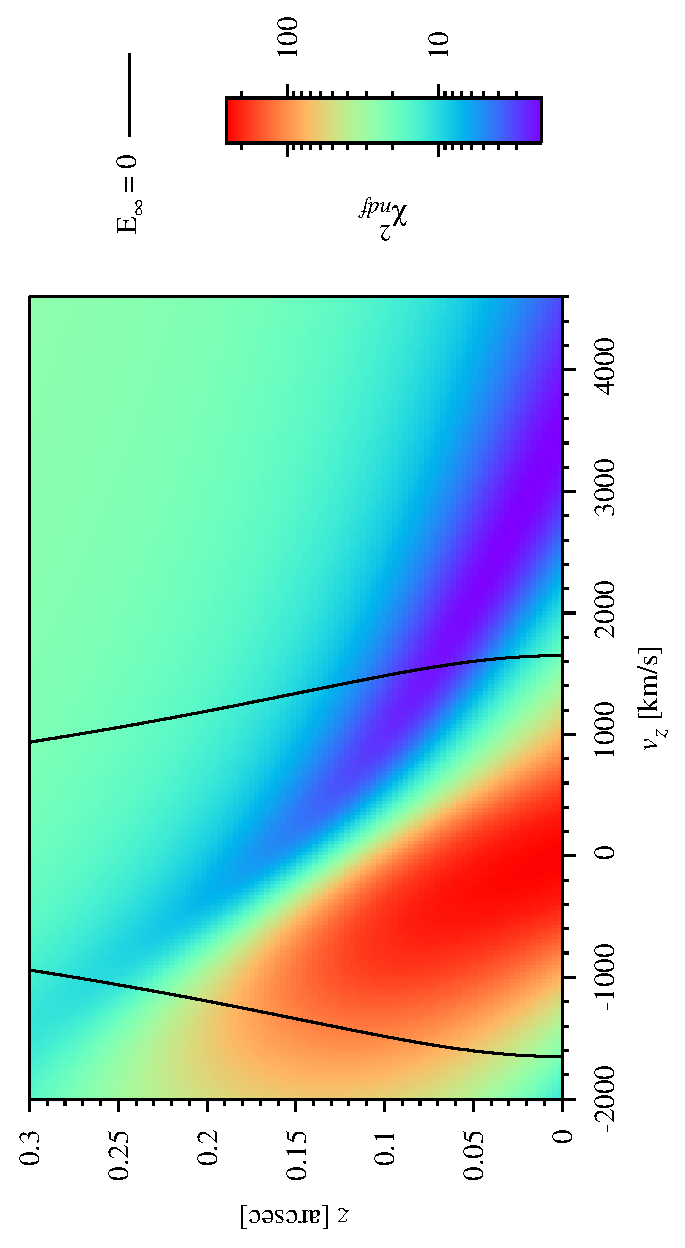
\includegraphics[angle=-90,width=0.9\textwidth]{eps/so1-BH-run3.eps}
	\caption{$\chi^2_{ndf}$ phase space plot for S0-1 with black hole. The lines represent the escape velocity required of the $v_z$
	component only, bound orbits being within the lines and unbound orbits outside. Epoch 1992.7.}
	\label{fig_so1BHphasespace}
	\end{center}
\end{figure}
\begin{figure}[!pb]
	\begin{center}
	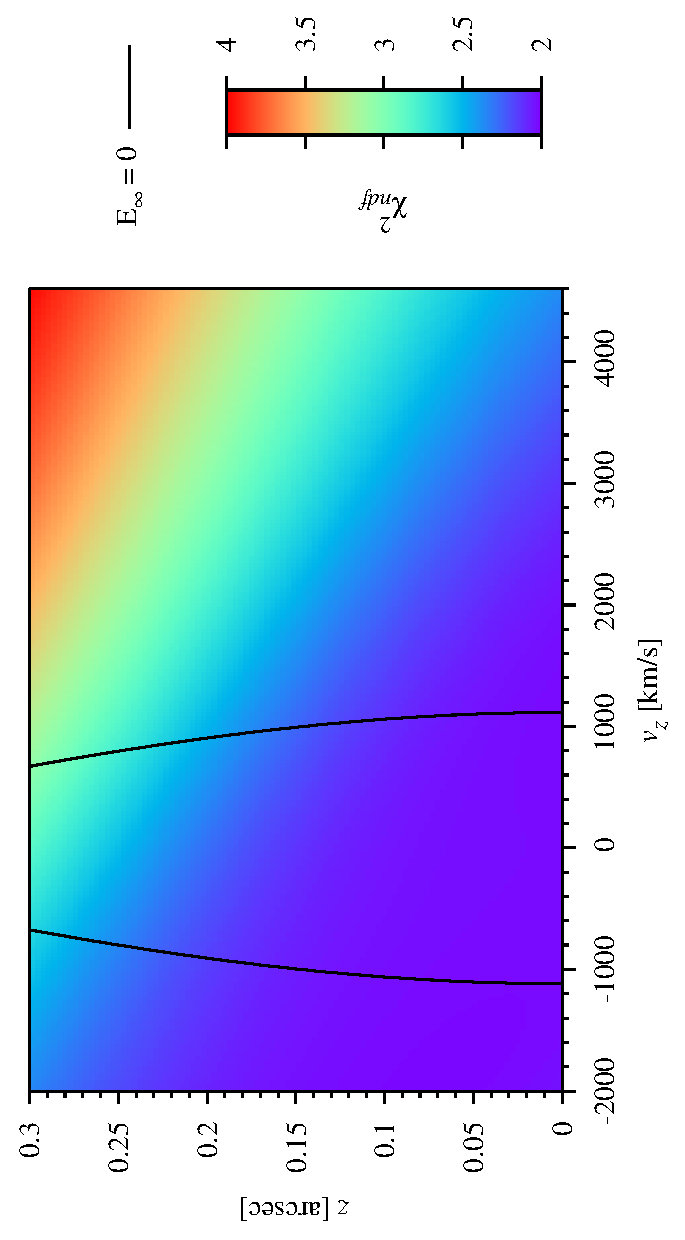
\includegraphics[angle=-90,width=0.9\textwidth]{eps/so1-FB-run9.eps}
	\caption{$\chi^2_{ndf}$ phase space plot for S0-1 with fermion ball. Epoch 1992.7.}
	\label{fig_so1FBphasespace}
	\end{center}
\end{figure}
\begin{figure}[!pt]
	\begin{center}
	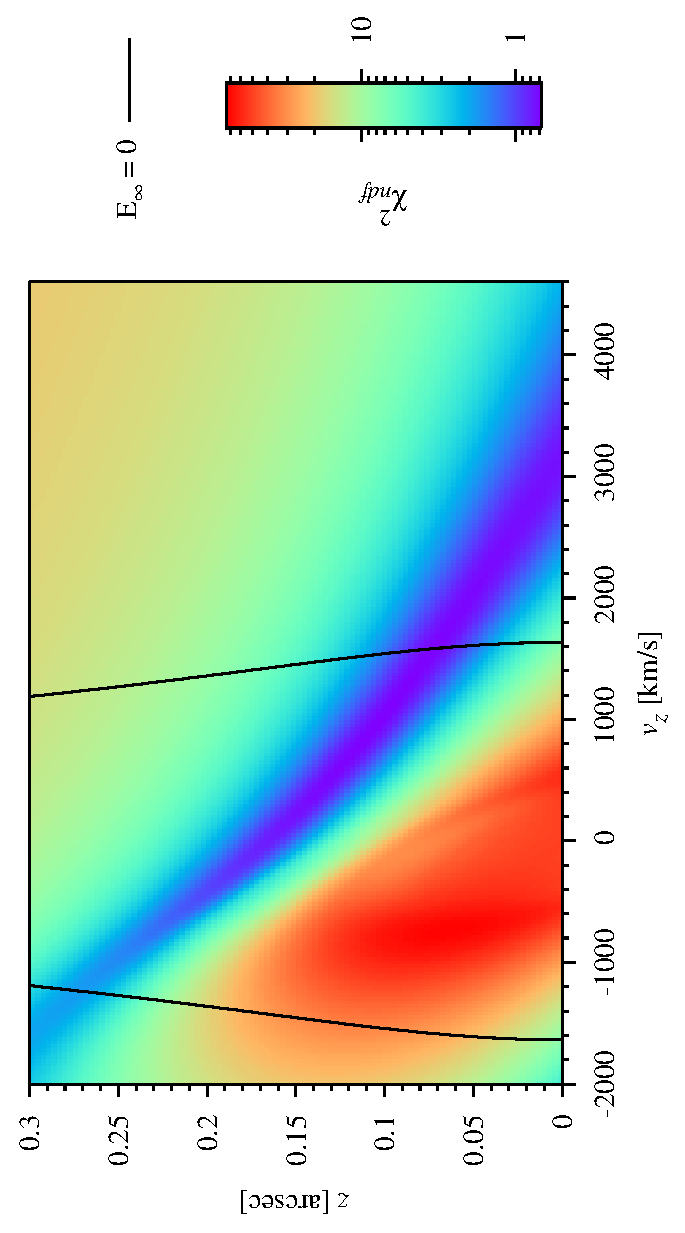
\includegraphics[angle=-90,width=0.9\textwidth]{eps/so2-BH-run2.eps}
	\caption{$\chi^2_{ndf}$ phase space plot for S0-2 with black hole. Epoch 1992.7.}
	\label{fig_so2BHphasespace}
	\end{center}
\end{figure}
\begin{figure}[!pb]
	\begin{center}
	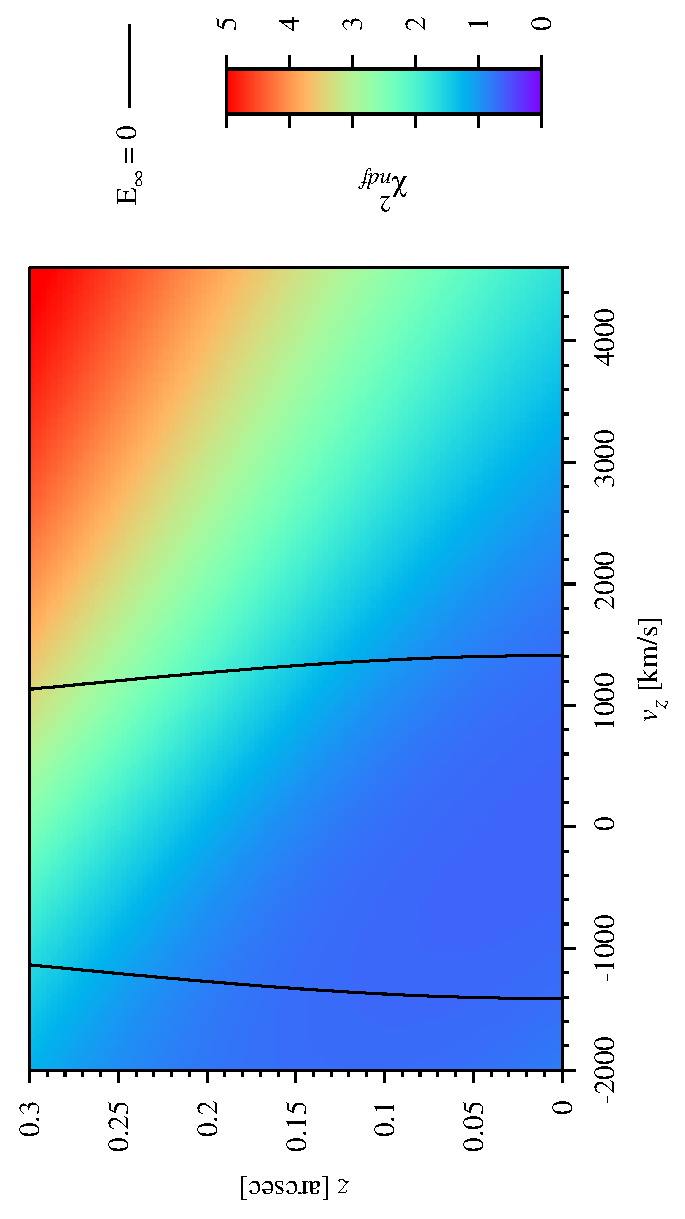
\includegraphics[angle=-90,width=0.9\textwidth]{eps/so2-FB-run9.eps}
	\caption{$\chi^2_{ndf}$ phase space plot for S0-2 with fermion ball. Epoch 1992.7.}
	\label{fig_so2FBphasespace}
	\end{center}
\end{figure}
\begin{figure}[!pt]
	\begin{center}
	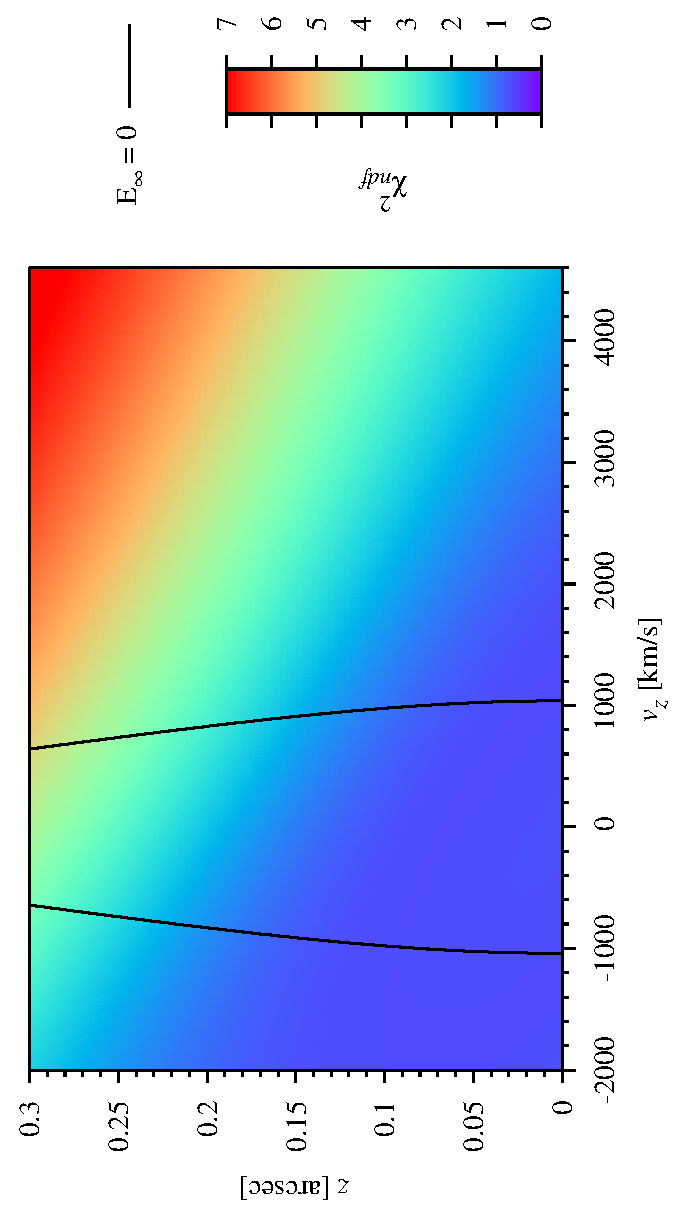
\includegraphics[angle=-90,width=0.9\textwidth]{eps/so4-BH-run2.eps}
	\caption{$\chi^2_{ndf}$ phase space plot for S0-4 with black hole. Epoch 1992.7.}
	\label{fig_so4BHphasespace}
	\end{center}
\end{figure}
\begin{figure}[!pt]
	\begin{center}
	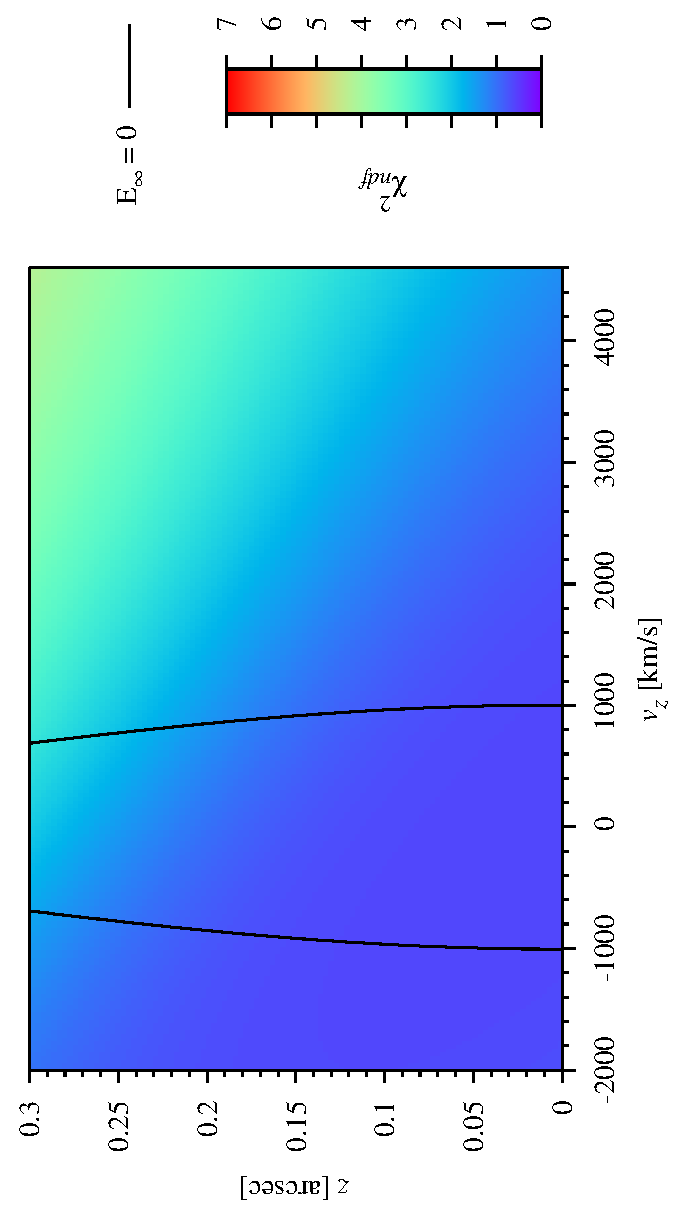
\includegraphics[angle=-90,width=0.9\textwidth]{eps/so4-FB-run9.eps}
	\caption{$\chi^2_{ndf}$ phase space plot for S0-4 with fermion ball. Epoch 1992.7.}
	\label{fig_so4FBphasespace}
	\end{center}
\end{figure}
\clearpage

\subsection{Analysis}
It is quite clear from Figures \ref{fig_so1BHphasespace} through \ref{fig_so4FBphasespace} that the fermion ball scenario applies 
much less constraints with selection of $z$ and $v_z$ initial conditions than the black hole scenario, which has quite rigid constraints.
Accurate
measurements of these parameters would most certainly be able to show if the black hole scenario describes the orbits sufficiently.
However, experimental complications in taking said measurements make this an unlikely method of discernment in the near future.

Due to the alikeness of Figures \ref{fig_so4BHphasespace} and \ref{fig_so4FBphasespace}, we can clearly see that phase space analysis on
S0-4 is unlikely to
be able to tell us much about the mass structure of the galactic centre. As the star would be located on the outer edge of the fermion ball,
the enclosed mass is almost that of the black hole, and the resulting dynamics are therefore very similar to those of the black hole scenario.
However, if S0-4 re-enters the fermion ball, a precessing orbit will be produced, and this will be observable over time. Also, it is
possible that S0-4 may travel incredibly close (within a milliparsec) of the black hole during the course of its orbit, for
Figure \ref{fig_so1bestfitssky} this occurs at around 2047. It may then be possible to observe relativistic effects upon
the star's spectra, assuming the technology to resolve these spectra will improve by that time. Obviously these effects would not be
present in the fermion ball scenario.

Observing the orbits of S0-1 and S0-2 will most certainly be a way to tell whether the galactic centre is a point source (black hole) or
an extended source. Unfortunately, the observations need to be made over a much longer timescale in order to see possible orbital precession.
S0-2 appears to show promise more quickly, allowing for discernment of any $z$-$v_z$ combination within a maximum of 30 years.
Data for $z$ and $v_z$ would certainly aid this process, and dramatically reduce the required observing time.
\begin{table}[!p]
	\begin{center}
	\begin{tabular}{c c c c c c c c c}
	\hline
	\hline
	Star & $x$ & $v_x$ & $y$ & $v_y$ & $z$ & $v_z$ & $\chi^2_{ndf}$ & Orbit \\
	\hline
	S0-1 BH &  0.125 & 0    & 0.105  & -900  & 0.012 & 3190  & 2.06 & unbound \\
	S0-1 FB &  0.121 & -200 & 0.110  & -1080 & 0.072 & -1940 & 2.02 & unbound \\
	S0-2 BH & -0.028 & 300  & 0.200  & -300  & 0.099 & 1090  & 0.68 & bound \\
	S0-2 FB & -0.028 & 300  & 0.200  & -450  & 0.000 & 40    & 0.65 & bound \\
	S0-4 BH & -0.250 & -800 & -0.120 & -600  & 0.000 & -1190 & 0.68 & unbound \\
	S0-4 FB & -0.250 & -760 & -0.116 & -600  & 0.072 & -410  & 0.65 & bound \\
	\hline
	\end{tabular}
	\end{center}
	\caption{Minimal $\chi^2_{ndf}$ for orbits of stars near the galactic centre. Final column notes a bound or unbound
	orbit using the escape velocity for that scenario, the number of degrees of freedom is 29. Positions 
	are in arcsec and velocities, km/s. All initial parameters are for epoch 1992.7 and for a mass of
	$2.6 \times 10^6 M_\odot$.}
	\label{tab_minimalzvzchisquare}
\end{table}
\begin{table}[!p]
	\begin{center}
	\begin{tabular}{c c c c c c c c c}
	\hline
	\hline
	Star & $x$ & $v_x$ & $y$ & $v_y$ & $z$ & $v_z$ & $\chi^2_{ndf}$ & Orbit \\
	\hline
	S0-1 BH &  0.125 & 0    & 0.105  & -900  & 0.000 & 3220  & 2.06 & unbound \\
	S0-1 FB &  0.121 & -200 & 0.110  & -1080 & 0.000 & 40    & 2.10 & bound \\
	S0-2 BH & -0.028 & 300  & 0.200  & -300  & 0.087 & 1120  & 0.68 & bound \\
	S0-2 FB & -0.028 & 300  & 0.200  & -450  & 0.000 & 40    & 0.83 & bound \\
	S0-4 BH & -0.250 & -800 & -0.120 & -600  & 0.000 & 40    & 0.69 & bound \\
	S0-4 FB & -0.250 & -760 & -0.116 & -600  & 0.000 & 40    & 0.70 & bound \\
	\hline
	\end{tabular}
	\end{center}
	\caption{Minimal $\chi^2_{ndf}$ for orbits of stars near the galactic centre of mass $2.4 \times 10^6 M_\odot$.}
	\label{tab_minimalzvzchisquareminmass}
\end{table}
\begin{table}[!p]
	\begin{center}
	\begin{tabular}{c c c c c c c c c}
	\hline
	\hline
	Star & $x$ & $v_x$ & $y$ & $v_y$ & $z$ & $v_z$ & $\chi^2_{ndf}$ & Orbit \\
	\hline
	S0-1 BH &  0.125 & 0    & 0.105  & -900  & 0.024 & 3130  & 2.07 & unbound \\
	S0-1 FB &  0.121 & -200 & 0.110  & -1080 & 0.000 & 2170  & 2.00 & unbound \\
	S0-2 BH & -0.028 & 300  & 0.200  & -300  & 0.111 & 1060  & 0.68 & bound \\
	S0-2 FB & -0.028 & 300  & 0.200  & -450  & 0.150 & -860  & 0.63 & bound \\
	S0-4 BH & -0.250 & -800 & -0.120 & -600  & 0.030 & 1450  & 0.68 & unbound \\
	S0-4 FB & -0.250 & -760 & -0.116 & -600  & 0.159 & -650  & 0.65 & bound \\
	\hline
	\end{tabular}
	\end{center}
	\caption{Minimal $\chi^2_{ndf}$ for orbits of stars near the galactic centre of mass $2.8 \times 10^6 M_\odot$.}
	\label{tab_minimalzvzchisquaremaxmass}
\end{table}
\begin{figure}[!p]
	\begin{center}
	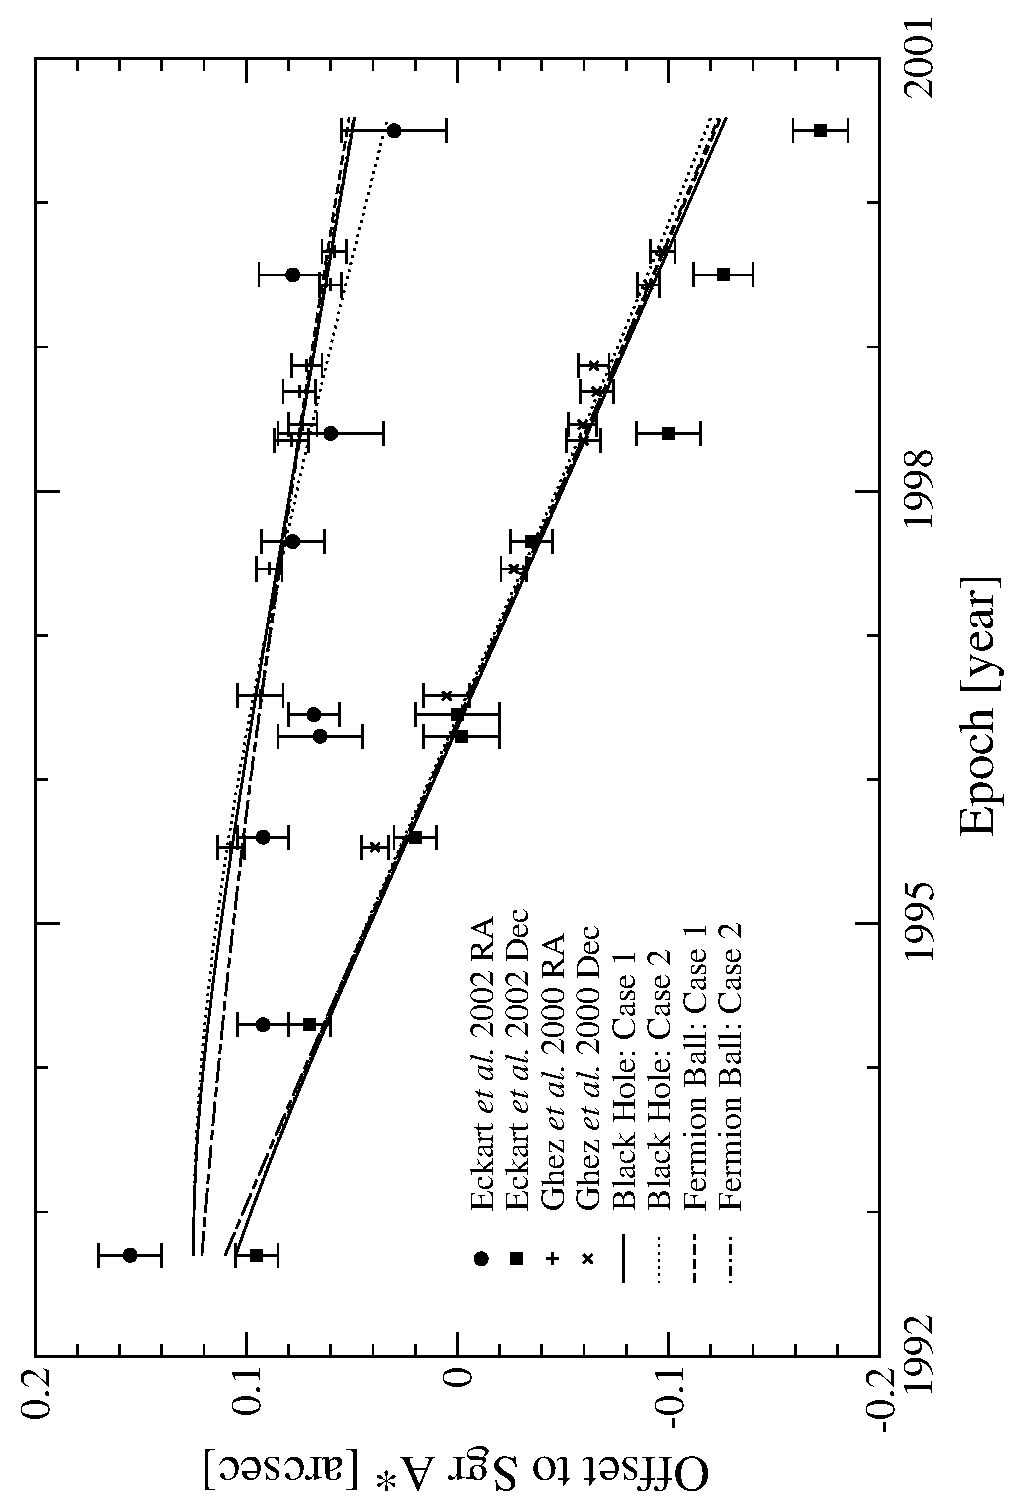
\includegraphics[angle=-90,width=0.9\textwidth]{eps/bestfits-so1.eps}
	\caption{Best fits for S0-1.
	``Black Hole: Case 1'' has $z$=0.012arcsec, $v_z$=3190km/s with an unbound orbit and $\chi^2_{ndf}=2.06$.
	``Black Hole: Case 2'' has $z$=0.075arcsec, $v_z$=1360km/s with a bound orbit and $\chi^2_{ndf}=2.54$.
	``Fermion Ball: Case 1'' has $z$=0.072arcsec, $v_z$=-1940km/s with an unbound orbit and $\chi^2_{ndf}=2.02$.
	``Fermion Ball: Case 2'' has $z$=0arcsec, $v_z$=0km/s with a bound orbit and $\chi^2_{ndf}=2.03$.}
	\label{fig_so1bestfits}
	\end{center}
\end{figure}
\begin{figure}[!p]
	\begin{center}
	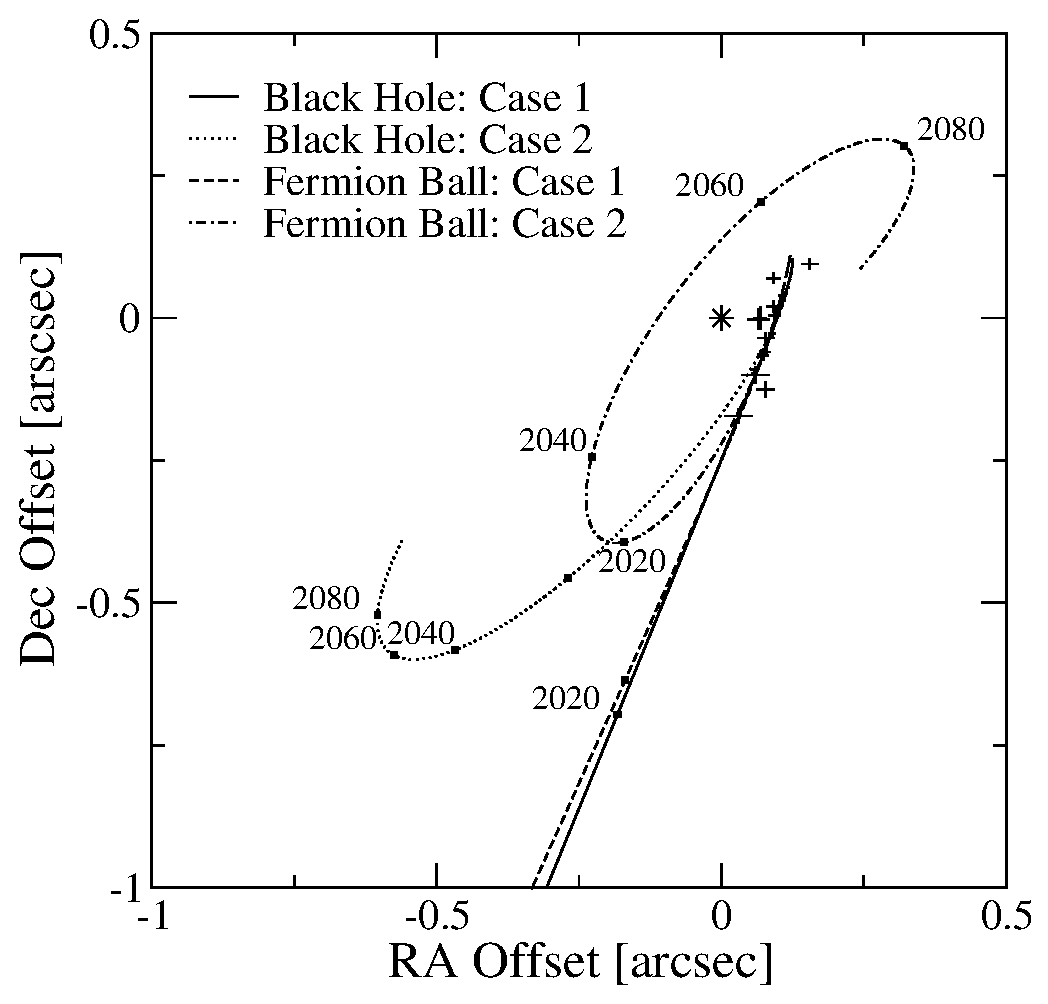
\includegraphics[width=0.9\textwidth]{eps/skyplot-so1.eps}
	\caption{Best fits for S0-1, sky-plot projected until 2100. All cases carry the same initial conditions as
	Figure \ref{fig_so1bestfits}. The dynamic location of Sgr A* is denoted by the star.}
	\label{fig_so1bestfitssky}
	\end{center}
\end{figure}
\begin{figure}[!p]
	\begin{center}
	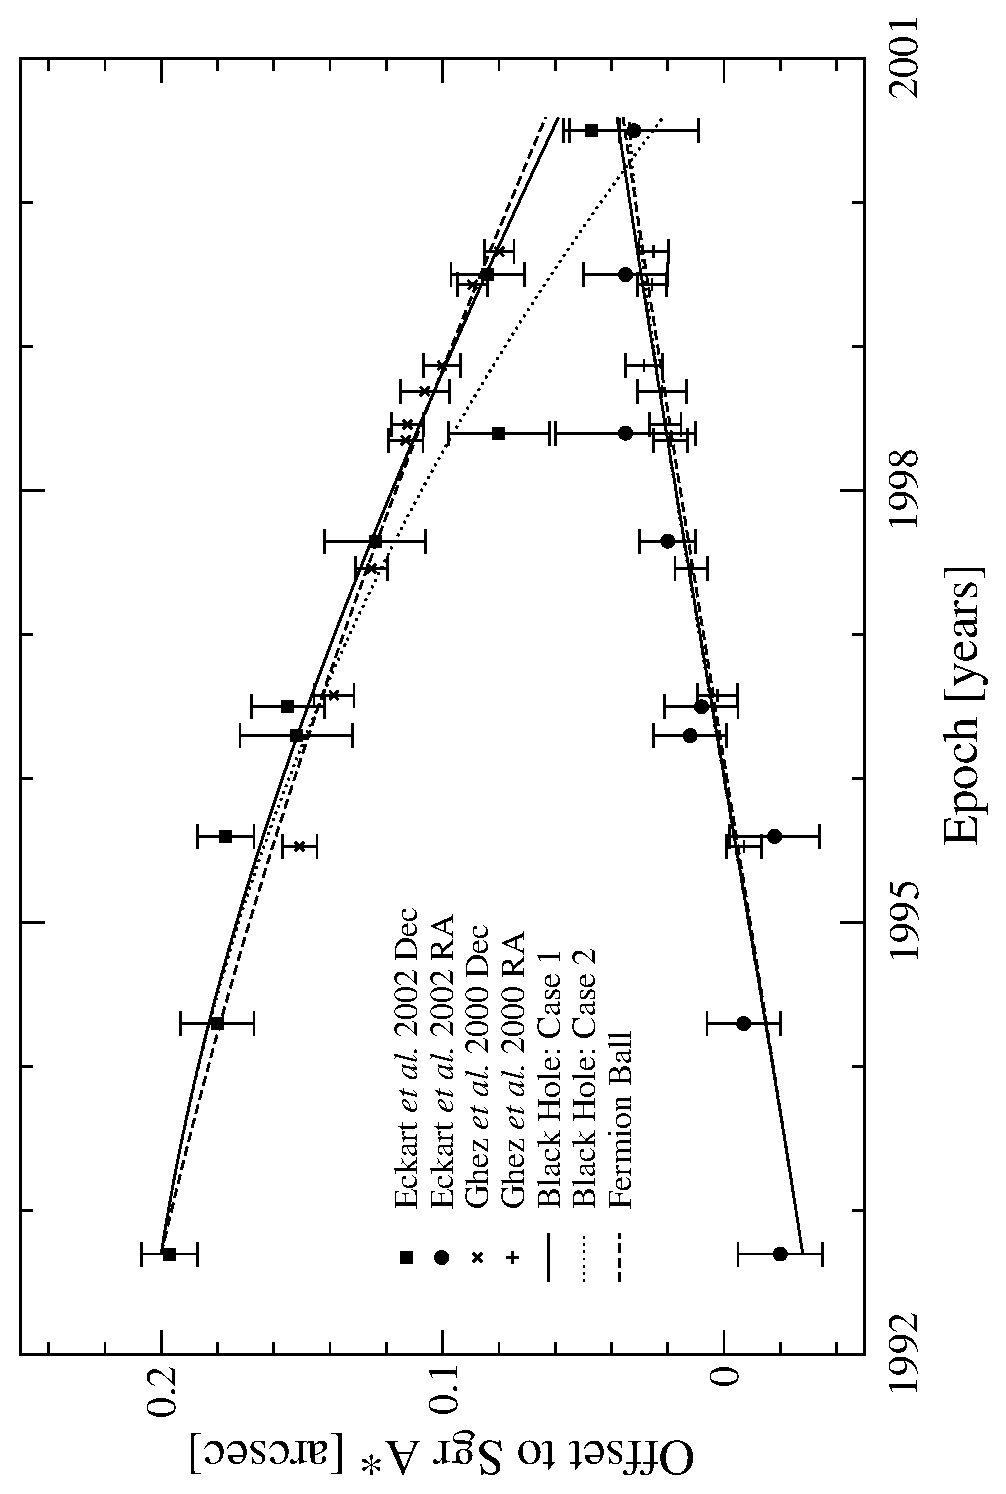
\includegraphics[angle=-90,width=0.9\textwidth]{eps/bestfits-so2.eps}
	\caption{Best fits for S0-2.
	``Black Hole: Case 1'' has $z$=0.099arcsec, $v_z$=1090km/s with a bound orbit and $\chi^2_{ndf}=0.68$.
	``Black Hole: Case 2'' has $z$=0.099arcsec, $v_z$=500km/s with a bound orbit and $\chi^2_{ndf}=3.27$.
	``Fermion Ball'' has $z$=0arcsec, $v_z$=40km/s with a bound orbit and $\chi^2_{ndf}=0.65$.
	``Black Hole: Case 2'' has been chosen in order to describe a very tight orbit around Sgr A*.}
	\label{fig_so2bestfits}
	\end{center}
\end{figure}
\begin{figure}[!p]
	\begin{center}
	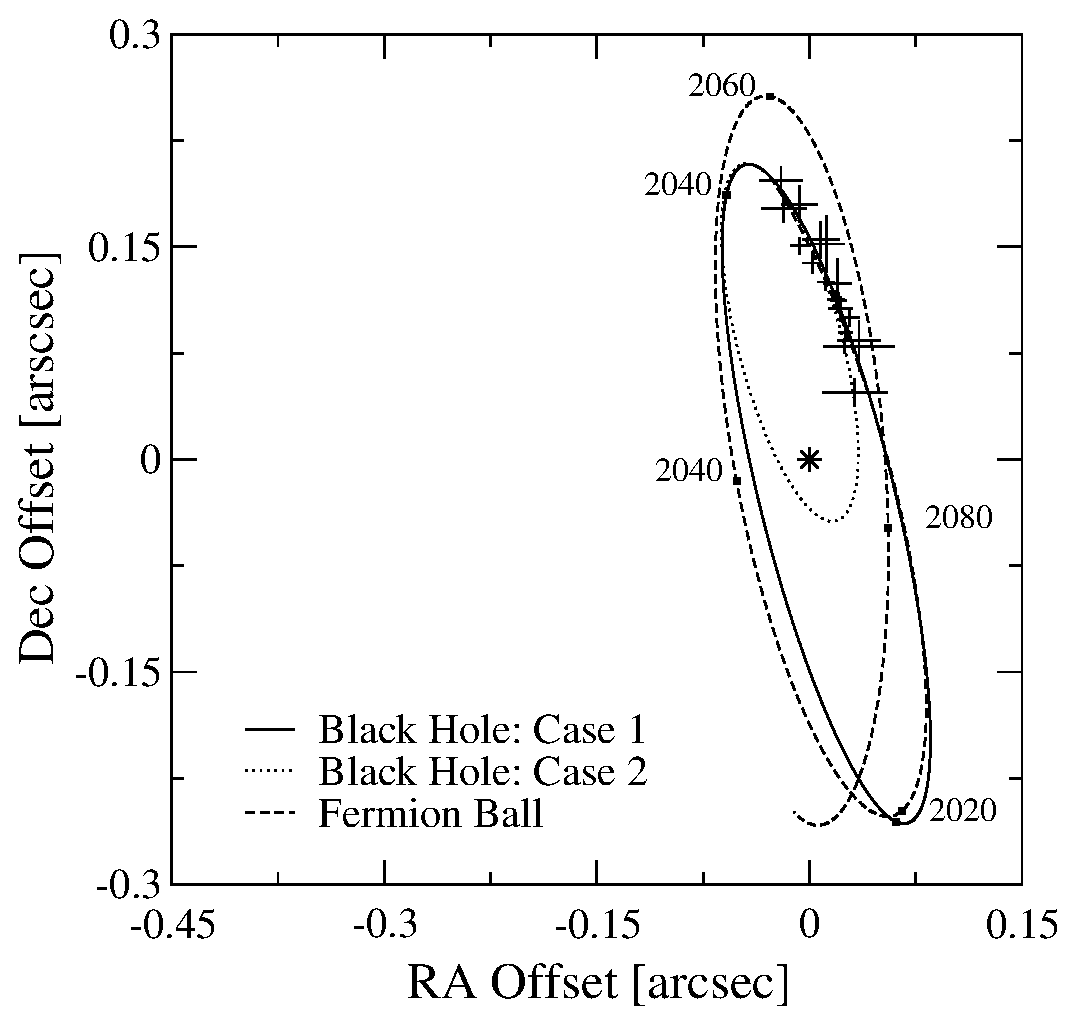
\includegraphics[width=0.9\textwidth]{eps/skyplot-so2.eps}
	\caption{Best fits for S0-2, sky-plot projected until 2100. All cases carry the same initial conditions as
	Figure \ref{fig_so2bestfits}. The black hole case 1 has a bound orbital period of 50 years, case 2 of 20 years.
	The dynamic location of Sgr A* is denoted by the star.}
	\label{fig_so2bestfitssky}
	\end{center}
\end{figure}
\begin{figure}[!p]
	\begin{center}
	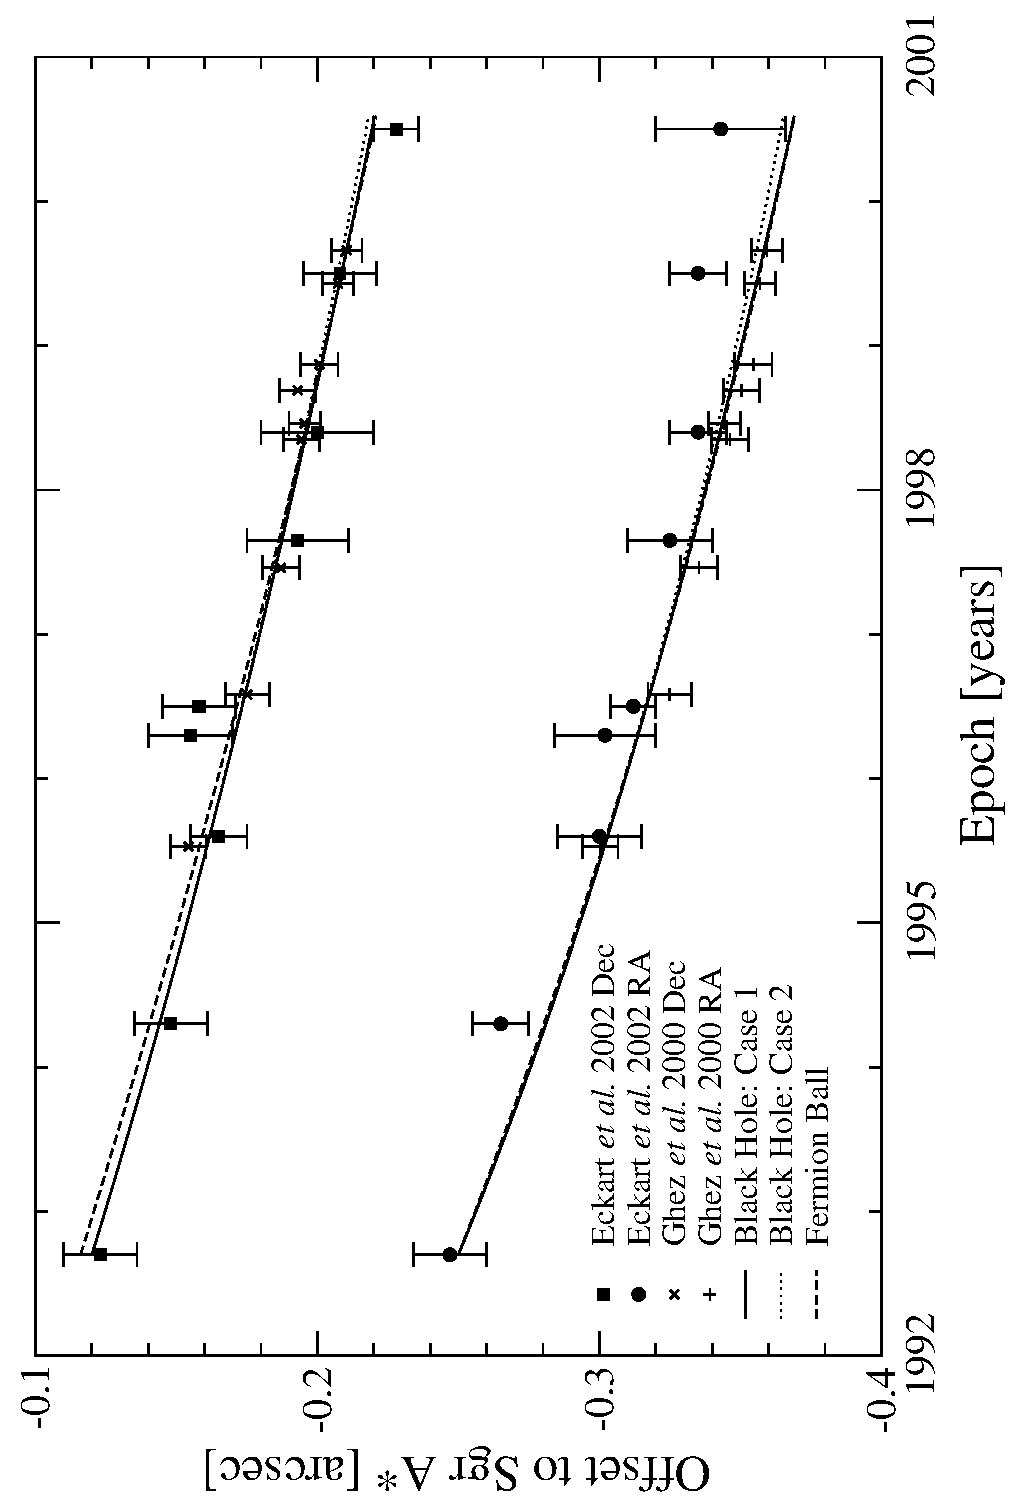
\includegraphics[angle=-90,width=0.9\textwidth]{eps/bestfits-so4.eps}
	\caption{Best fits for S0-4.
	``Black Hole: Case 1'' has $z$=0arcsec, $v_z$=-1190km/s with an unbound orbit and $\chi^2_{ndf}=0.68$.
	``Black Hole: Case 2'' has $z$=0arcsec, $v_z$=0km/s with a bound orbit of $\chi^2_{ndf}=0.72$.
	The ``Fermion Ball'' case has $z$=0.072arcsec, $v_z$=-410km/s with a bound orbit and $\chi^2_{ndf}=0.65$.}
	\label{fig_so4bestfits}
	\end{center}
\end{figure}
\begin{figure}[!p]
	\begin{center}
	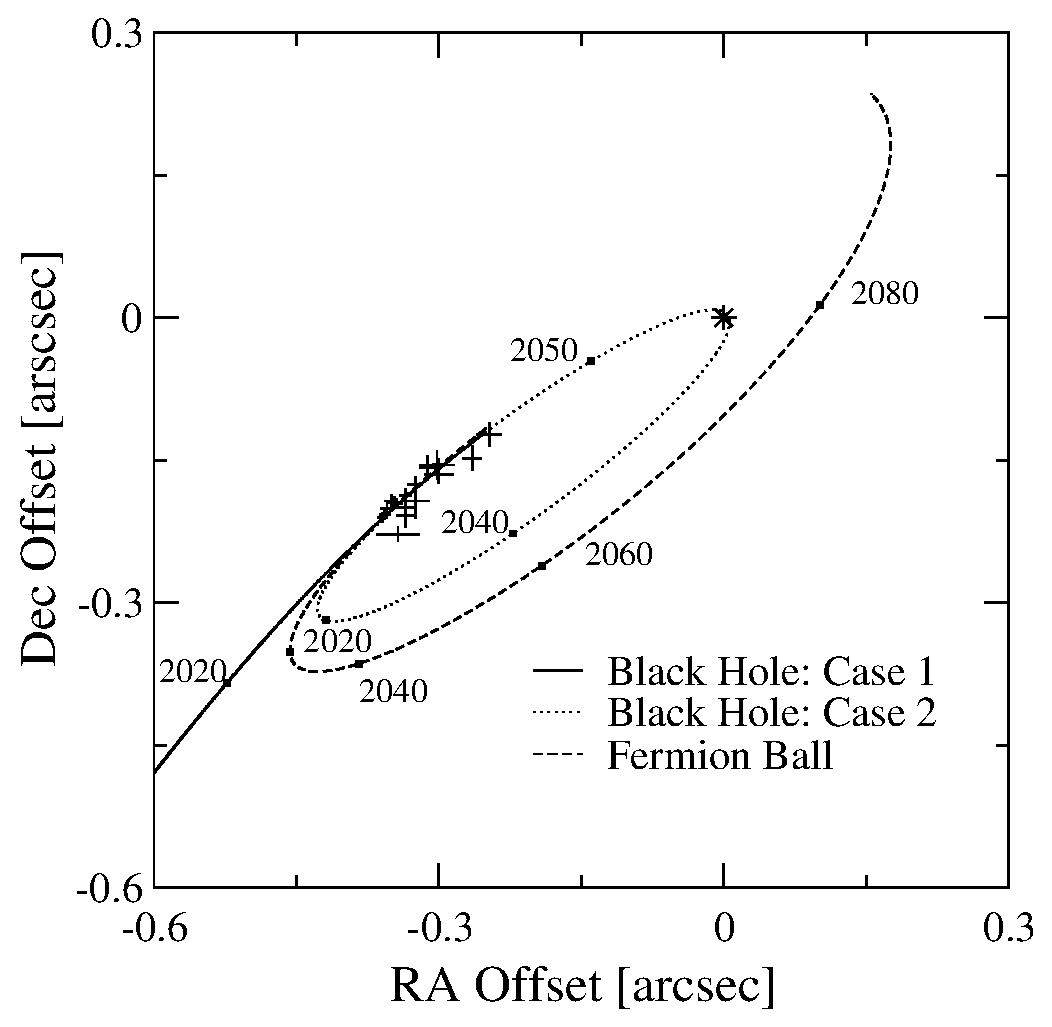
\includegraphics[width=0.9\textwidth]{eps/skyplot-so4.eps}
	\caption{Best fits for S0-4, sky-plot projected until 2100. All cases carry the same initial conditions as
	Figure \ref{fig_so4bestfits}. ``Black Hole: Case 2'' has a bound orbital period of 60 years. The dynamic
	location of Sgr A* is denoted by the star.}
	\label{fig_so4bestfitssky}
	\end{center}
\end{figure}
\clearpage

\subsection{The Importance of $v_z$ and $z$}
\label{sec_futureps}
Since Newton's equations of motion (\ref{eqn_newtonmotion}) are time reflection invariant, it is possible to numerically solve the
orbital paths back-wards in time.
This allows for setting of initial parameters in any epoch. If accurate $z$ or $v_z$ data were to be made available in say 2005,
it would constrain the $\chi^2$ phase space plots for that epoch, dramatically reducing the required observing time needed
for distinguishing black hole or mass distribution.

Several phase space plots are now presented for epoch 2005 (Figures \ref{fig_so1-2005-run2} and \ref{fig_so2-2005-run1}),
with initial parameters projected from the $\chi^2$ reduction in Section \ref{bestfits}.
However, data fitting is restricted to pre 2000.5 (the most recent observation) and we have therefore assumed
an orbital path up to our `initial' start date of 2005.

It is clear from these plots that accurate $z$ and $v_z$ would instantly allow distinguishing between the 2 scenarios.
\begin{figure}[!p]
	\begin{center}
	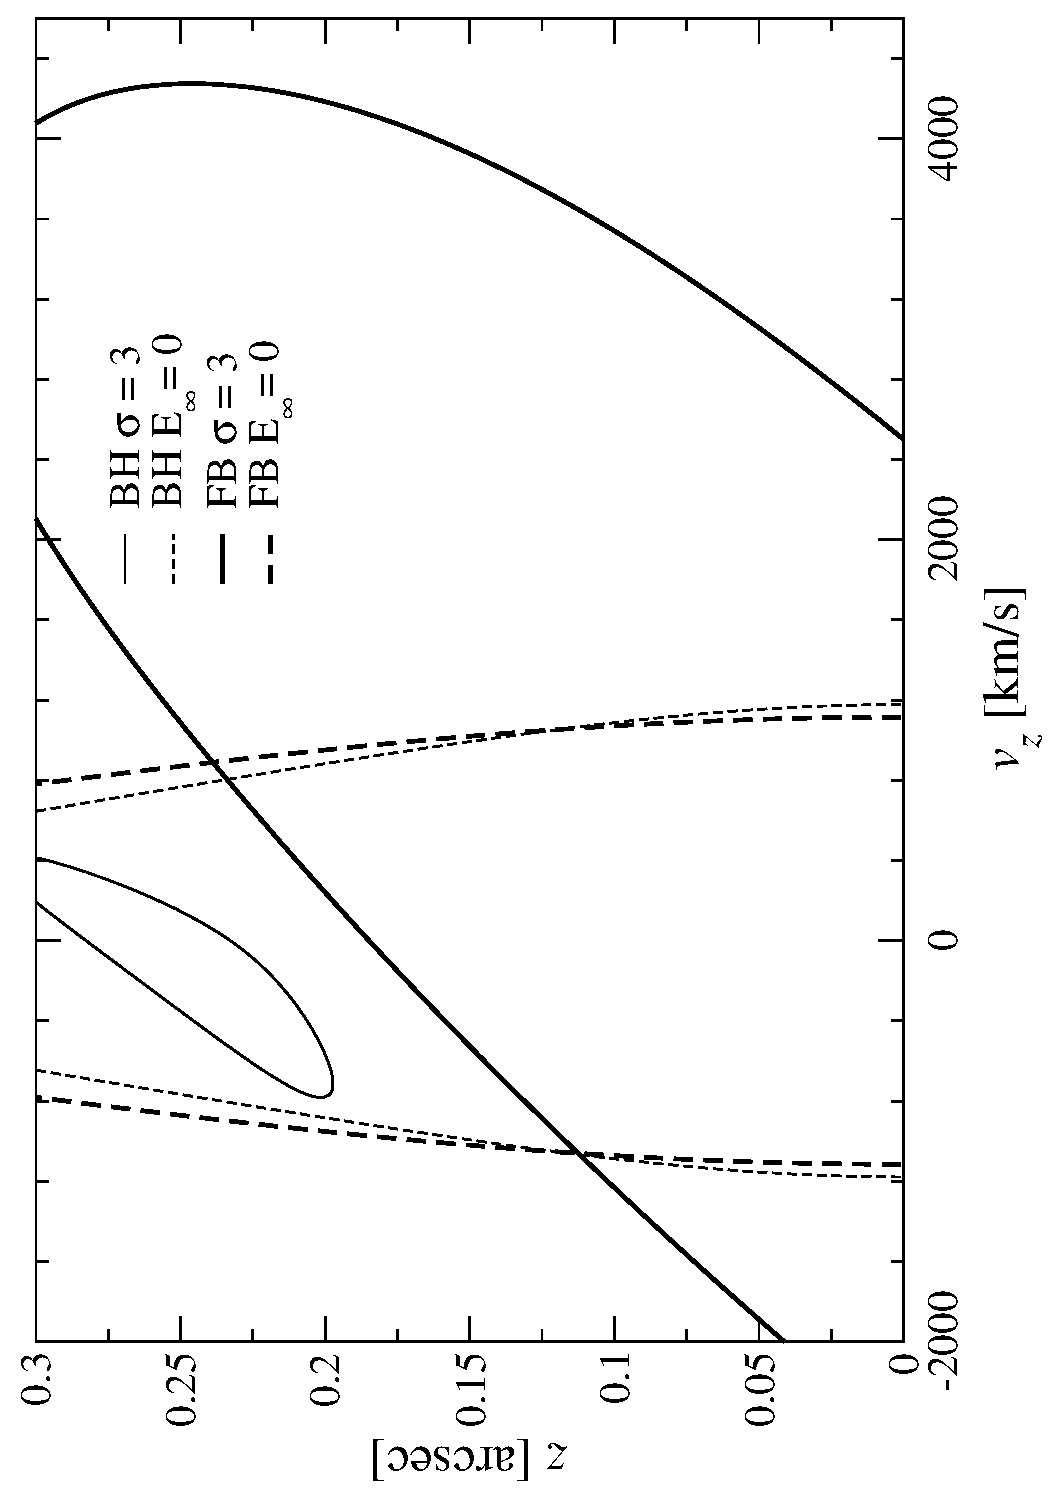
\includegraphics[angle=-90,width=0.9\textwidth]{eps/phasespace-2005-run2-so1.eps}
	\caption{$\chi^2_{ndf}$ phase space plot for S0-1 at epoch 2005. The paths for both ``Case 2'' scenarios in Figure
	\ref{fig_so1bestfits} have been used to give the `initial' position and velocity parameters for this plot (therefore we have
	assumed a bound orbit), values are in Table \ref{tab_so1-2005-run2}.
	Contour lines for $\chi^2_{ndf}$=3 are shown for both black hole and fermion ball scenarios, alongside
	the corresponding escape velocities.
	It is clear that the minimal $\chi^2_{ndf}$ values for each scenario occupy different regions
	and therefore an accurate measurement of $z$ or $v_z$ would instantly allow one of the scenarios to be eliminated. For example a
	$z$ measurement of 0.05arcsec would disallow the black hole scenario, similarly a $z$ measurement of 0.25arcsec and $v_z$
	of 0km/s would rule out the fermion ball scenario.}
	\label{fig_so1-2005-run2}
	\end{center}
\end{figure}
\begin{table}[!p]
	\begin{center}
	\begin{tabular}{c c c c c}
	\hline
	\hline
	Scenario & $x$ & $v_x$ & $y$ & $v_y$\\
	\hline
	BH &  -0.044 & -656  & -0.227 & -822 \\
	FB &  -0.007 & -492  & -0.233 & -811 \\
	\hline
	\end{tabular}
	\end{center}
	\caption{Initial parameters for Figure \ref{fig_so1-2005-run2}. Epoch 2005. Positions are in arcsec and velocities, km/s.}
	\label{tab_so1-2005-run2}
\end{table}
\clearpage
\begin{figure}[!p]
	\begin{center}
	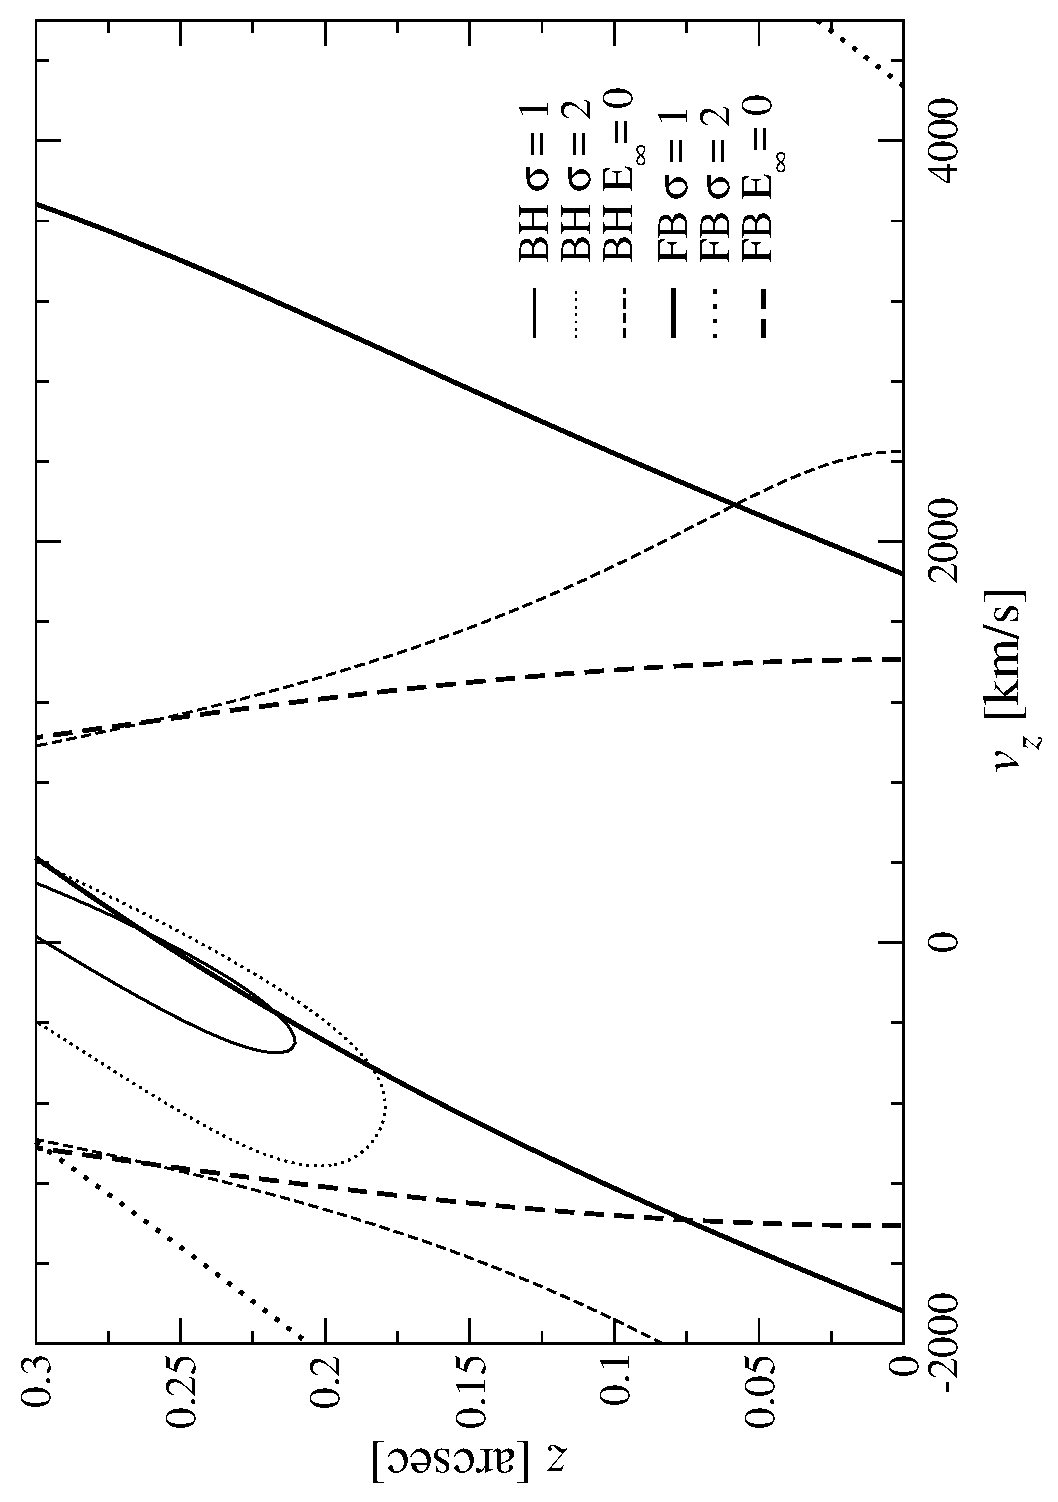
\includegraphics[angle=-90,width=0.9\textwidth]{eps/phasespace-2005-run1-so2.eps}
	\caption{$\chi^2_{ndf}$ phase space plot for S0-2 at epoch 2005. The minimal $\chi^2$ paths in Figure \ref{fig_so2bestfits}
	have been used to give the `initial' position and velocity parameters for this plot, values are in Table \ref{tab_so2-2005-run1}.
	Contour lines for $\chi^2_{ndf}$=1 and 2 are shown for both black hole and fermion ball scenarios, alongside the corresponding
	escape velocities.
	In this case, an accurate measurement of $z$ or $v_z$ may only allow for elimination of the black hole scenario, as the fermion ball
	minimal $\chi^2_{ndf}$ region is quite large.}
	\label{fig_so2-2005-run1}
	\end{center}
\end{figure}
\begin{table}[!p]
	\begin{center}
	\begin{tabular}{c c c c c}
	\hline
	\hline
	Scenario & $x$ & $v_x$ & $y$ & $v_y$\\
	\hline
	BH &  -0.067 & -196  & -0.050 & -922 \\
	FB &  -0.064 & -194  & -0.035 & -845 \\
	\hline
	\end{tabular}
	\end{center}
	\caption{Initial parameters for Figure \ref{fig_so2-2005-run1}. Epoch 2005. Positions are in arcsec and velocities, km/s.}
	\label{tab_so2-2005-run1}
\end{table}
